% !TEX TS-program = lualatex
% !TEX encoding = UTF-8 Unicode

% This is a simple template for a LaTeX document using the "article" class.
% See "book", "report", "letter" for other types of document.

\documentclass[10pt, twocolumn]{article} % use larger type; default would be 10pt

\usepackage[utf8]{inputenc} % set input encoding (not needed with XeLaTeX)
\usepackage{fontspec}
\setmainfont{Georgia}
\setsansfont{Georgia}
\setmonofont{Georgia}
%\usepackage[none]{hyphenat}
\usepackage{hyphenat}

%%% Examples of Article customizations
% These packages are optional, depending whether you want the features they provide.
% See the LaTeX Companion or other references for full information.

%%% PAGE DIMENSIONS
\usepackage{geometry} % to change the page dimensions
\geometry{a4paper, left=17.5mm, right=17.5mm, textwidth=85mm,columnsep=5mm, top=17.5mm}
\setlength{\parindent}{0pt}
% or letterpaper (US) or a5paper or....
% \geometry{margin=2in} % for example, change the margins to 2 inches all round
% \geometry{landscape} % set up the page for landscape
%   read geometry.pdf for detailed page layout information

\usepackage{subcaption}
\usepackage{graphicx} % support the \includegraphics command and options

\usepackage[parfill]{parskip} % Activate to begin paragraphs with an empty line rather than an indent

%%% PACKAGES
\usepackage{booktabs} % for much better looking tables
\usepackage{array} % for better arrays (eg matrices) in maths
\usepackage{paralist} % very flexible & customisable lists (eg. enumerate/itemize, etc.)
\usepackage{verbatim} % adds environment for commenting out blocks of text & for better verbatim
%\usepackage{subfig} % make it possible to include more than one captioned figure/table in a single float
\usepackage{amsmath}
% These packages are all incorporated in the memoir class to one degree or another...
\usepackage{lipsum}
%\usepackage{caption}
\usepackage{listings}

%%% HEADERS & FOOTERS
\usepackage{fancyhdr} % This should be set AFTER setting up the page geometry
\pagestyle{fancy} % options: empty , plain , fancy
\renewcommand{\headrulewidth}{0pt} % customise the layout...
\lhead{}\chead{}\rhead{}
\lfoot{}\cfoot{\thepage}\rfoot{}

%%% SECTION TITLE APPEARANCE
%\usepackage{sectsty}
%\allsectionsfont{\sffamily\mdseries\upshape} % (See the fntguide.pdf for font help)
% (This matches ConTeXt defaults)

%%% ToC (table of contents) APPEARANCE
\usepackage[nottoc,notlof,notlot]{tocbibind} % Put the bibliography in the ToC
\usepackage[titles,subfigure]{tocloft} % Alter the style of the Table of Contents
\renewcommand{\cftsecfont}{\rmfamily\mdseries\upshape}
\renewcommand{\cftsecpagefont}{\rmfamily\mdseries\upshape} % No bold!
\usepackage{authblk}

\usepackage{float}

\newcommand{\overbar}[1]{\mkern 1.5mu\overline{\mkern-1.5mu#1\mkern-1.5mu}\mkern 1.5mu}

%%% END Article customizations

%%% The "real" document content comes below...

\title{\textbf{Investigation of fractal dimension in modified diffusion-limited aggregation algorithms}}
\author{Candidate Number: 24669}
\affil{Department of Physics, University of Bath, Bath BA2 7AY, United Kingdom}
%\date{} % Activate to display a given date or no date (if empty),
         % otherwise the current date is printed 

\begin{document}
\twocolumn[
 \begin{@twocolumnfalse}
\maketitle
\begin{abstract}
  Following observation of unconventional superconductive effects in twisted bilayer graphene, the novel field of 'twistronics' has seen a rapid progression in theory and experiment. When a Van der Vaals heterostructure formed from a bilayer of 2D lattices is twisted at a so-called 'magic-angle' perturbation effects and interlayer tunneling lead to the formation of a flat electronic band at fermi level in some materials. These exotic electronic properties have the potential to be exploited as high temperature superconductors or in novel electronic devices. Using a multiorbital tight binding model (TBM) we model a bilayer of transition metal dichalcogenide 2H-NbSe$_2$ with interlayer tunneling at various twist angles. We observe ***** in the electronic band structure at *** points. Our results show potential for further modelling of the NbSe$_2$.

\bigskip
\end{abstract}
\end{@twocolumnfalse}
]
\medskip

\section*{Introduction}

  In 2018 Cao Y. et al\cite{Cao_2018} realised unconventional superconductivity in bilayer graphene twisted to the 'magic-angle' of 1.1$^\circ$ 


\section*{Method}
  Our work draws on several published methods on NbSe2 and twistronics. In particular we take the multiorbital tight binding model of monolayer NbSe2 from Habara and Wakabayashi\cite{Habara_2021}. To model the bilayer with twist, we employ the method used in the original magic-angle paper by Bistritzer and MacDonald \cite{Bistritzer_2011}. 

\subsection*{Monolayer NbSe2}
  We employ a multiorbital tight binding model (TBM) of NbSe2 as described by Habara and Wakabayashi \cite{Habara_2021}. We take a basis of the 3 d orbitals of the Nb atoms with spin orbit coupling. These states are dominant in the electronic band near fermi level. We take this as an adequate description of the NbSe$_2$ monolayer for low energy electronic states.

  The TBM takes the interactions of these states up to the third nearest neighbour sites.

  The eigenvalue equation of the TBM is 
      \begin{equation}
        \label{TBM_evalue_eqn}
        \hat{H}(\boldsymbol{k})\left|u_{n k}\right\rangle=E_{n k}\left|u_{n k}\right\rangle,
      \end{equation}

   where $k=\left(k_{x}, k_{y}\right)$ is the wave-number vector, $E_{nk}$ is the eigenvalue and $n = 1,2,\cdots,6$ is the band index.

   we define the eigenvectors as
      \begin{equation}
        \left|u_{n k}\right\rangle=$ $\left(c_{n k, d_{z^{2}}, \uparrow}, c_{n k, d_{x y}, \uparrow}, c_{n k, d_{x^{2}-y^{2}}, \uparrow}, c_{n k, d_{z^{2}}, \downarrow}, c_{n k, d_{x y}, \downarrow}, c_{n k, d_{x^{2}-y^{2}}, \downarrow}\right)^{T}
      \end{equation}

  where $(\cdots)^T$ indicates the transpose of the vector and $c_{nk\tau s}$ is the amplitude at atomic orbital $\tau$ with spin $s$ for the $n$th energy band at $k$.

  The monolayer hamiltonian $\hat{H}(\boldsymbol{k})$ with spin orbit coupling is then 
      \begin{equation}
        \hat{H}(\boldsymbol{k})=\hat{\sigma}_{0} \otimes \hat{H}_{\mathrm{TNN}}(\boldsymbol{k})+\hat{\sigma}_{z} \otimes \frac{1}{2} \lambda_{\mathrm{SOC}} \hat{L}_{z}
      \end{equation}

      with TBM nearest neighbour hamiltonian

      \begin{equation}
        \hat{H}_{\mathrm{TNN}}(\boldsymbol{k})=\left(\begin{array}{ccc}
        V_{0} & V_{1} & V_{2} \\
        V_{1}^{*} & V_{11} & V_{12} \\
        V_{2}^{*} & V_{12}^{*} & V_{22}
        \end{array}\right)
      \end{equation}

  and spin orbit coupling term

      \begin{equation}
        \hat{L}_{z}=\left(\begin{array}{ccc}
        0 & 0 & 0 \\
        0 & 0 & -2 i \\
        0 & 2 i & 0
        \end{array}\right)
      \end{equation}

  \item $\hat{\sigma}_0$ and $\hat{\sigma}_z$ are pauli matrices and $\lambda_{\text{SOC}}=0.0784$ eV is the Ising-type spin orbit coupling parameter. $V_0 \cdots V_{22}$ are functions of $k$ $^{[5]}$.

    The monolayer hamiltonian is then a 6x6 block diagonal hermitian matrix as a funciton of wavevector $k$.

    the eigenvalues of this hamiltonian correspond to the 6 eigenstates / electronic bands for a given point in reciprocal space $k$ 

  Specifically, we take $k$ from slices in the first brilloin zone along the standard critical points. By Bloch's theorem we can describe the electronic properties of the whole monolayer due to the periodic potentials.

  Further, due to reflectional symmetry the region that fully describes the electronic states can be reduced to the equilateral triangle bounded by $\Gamma \rightarrow K \rightarrow M \rightarrow K' \rightarrow \Gamma$.

\begin{figure}[t]
\centering
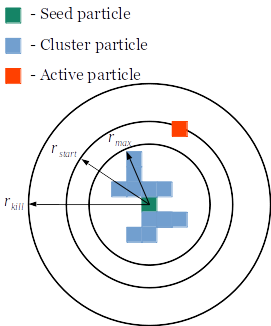
\includegraphics[width=0.95\columnwidth]{DLA_diagram.png}
  \caption{
    Diagram of the diffusion-limited aggregation (DLA) system. A particle is created at a random point on $r_{start}$ and then undergoes a discrete random walk. If its position exceeds the distance $r_{kill}$ it is removed. If it makes contact with the cluster it is made inactive and joins the cluster. The DLA cluster grows from an initial seed particle located at the origin, its size can be estimated from $r_{max}$.
  }
  \label{DLA_diagram}
\end{figure}

  Some approximations are made in this algorithm to improve computational efficiency. The original model described by Witten and Sander \cite{Witten_1981} removes particles when they reach the edge of the grid. However, this can result in significant computation spent on random walking a particle in the domain, only for it to walk to the edge and be removed. Further, if it does random walk back to a point on the circle $r_{start}$ its previous motion away from the cluster will not effect its subsequent motion. We therefore restrict the random walking to within $r_{kill}$ which still allows for some motion away from the cluster while improving overall efficiency. This restriction will have an effect on the resulting DLA cluster. However, we assume the effect is negligible for the reasons outlined.

  The random number sampling used for the random walk and the initial positions of particles generated on $r_{start}$ uses pseudo-random number generation to efficiently generate large quantities of random numbers. To ensure that the system does not generate the same cluster every time, a 'true' random number is used as the \textit{seed} of the pseudo-random number generater for each new cluster. This allows for the efficient sampling of many psuedo-random numbers that are independent between simulations, the resulting DLA clusters are consequently independent from one another.

\subsection*{Modified DLA - random adhesion}
  Previously we define \textit{checkStick()} to always be \textit{true}. However, in the modified algorithm as described by Ranguelov \textit{et al} \cite{Ranguelov_2011} we redefine \textit{checkStick()} to check against a preset probability of particle adherence $P_{stick}$, retrieving the unmodified algorithm for $P_{stick} = 1$. If the particle fails to adhere to the cluster it will do nothing until the next update where it will perform another random walk. An additional modification is made to the random walk procedure, such that if a particle tries to move into an occupied grid position it will not move and instead \textit{checkStick()} again. This prevents multiple particles from occupying a single grid space, and allows particles to have multiple 'chances' to adhere to the cluster at the same site.

\subsection*{Fractal dimension}
  A definition of dimension suitable to numerical computations of fractal dimension is the Minkowski-Bouligand or 'box-count' dimension: in a Euclidian space, the number of boxes $N$ (or 'density') with side length $a$ that cover a fractal of one dimensional size $R$ are related by
  \begin{equation}
      \begin{aligned}
        & N = (R/a)^{d_f}\\
        \implies & d_f = \frac{\ln(N)}{\ln(R/a)},
      \end{aligned}
      \label{dim_definition}
  \end{equation}

  where $d_f$ is the fractal dimension. With this definition we can retrieve well known dimensions such as $d_{line} = 1, d_{square} = 2$, etc.

      To determine the fractal dimension of the generated DLA clusters we first set $a=1$ as our DLA system is discrete in the grid, then $N=N_c$ is the number of particles in the cluster. We then assume that $r_{max}$ (the distance of the furthest point in the cluster from the origin) is representative of the one-dimensional size of the cluster with some correction terms $\alpha, \beta$. So our general relation is

  \begin{equation}
    \begin{aligned}
    & N_c(r_{max}) = (\alpha r_{max})^{d_f}+\beta\\
    \implies & \frac{d(\ln{N_c})}{d(\ln{r_{max}})} = \frac{d_f}{1 + \beta/(\alpha r_{max})^{d_f}}\\
    \implies & d_f = \lim\limits_{r_{max} \to \infty} \frac{d(\ln{N_c})}{d(\ln{r_{max}})},
    \end{aligned}
    \label{dim_relation}
  \end{equation}

  hence for sufficiently large $r_{max}$ relative to the length scale $a = 1$ we can estimate the fractal dimension $d_f$ of a DLA cluster. 

  Two methods are employed in the derivation of $d_f$ for individual DLA clusters: firstly a least squares fit method of the relationship described by (\ref{dim_relation}) is applied to the recorded values of $N_c$ and $r_{max}$ of the cluster, the corresponding $d_f$ is inferred from the fit with error; the second method approximates
  \begin{equation}
    d_f \approx \frac{\ln{N_c}}{\ln{r_{max}}}, \quad r_{max} \approx R >> a
    \label{dim_approx}
  \end{equation}
      by assuming that $r_{max}$ is sufficiently large for some $N_c$. $d_f$ is then found at the largest $N_c$ and corresponding $r_{max}$ that the cluster attains. The efficacy of these methods when applied is discussed with the results of this report.

\subsection*{Implementation}
  Please see the appendix for practical details about the specific implementation of the DLA algorithm used for this report.

\section*{Results and discussion}
  We make the assumtion that the distribution of $r_{max}$ and corresponding fractal dimension $d_f$ between many randomly sampled clusters is normal (by the central limit theorem \cite{Sadovnik_2016}) - allowing for the statistical treatment of error. Unless otherwise stated any uncertainties given will be the 95\% confidence interval on the mean. Please see the appendix for examples of clusters generated.

\subsection*{DLA cluster fractal dimension}
  Using the DLA system as described we can generate datasets from several DLA clusters of varying sizes. In particular a dataset of 100 clusters of $N_c = 20000$ particles is generated with recorded values of $N_c$ and $r_{max}$ as they grow. For this dataset and the analysis in this subsection we set $P_{stick} = 1$.

\begin{figure}[t!]
\centering
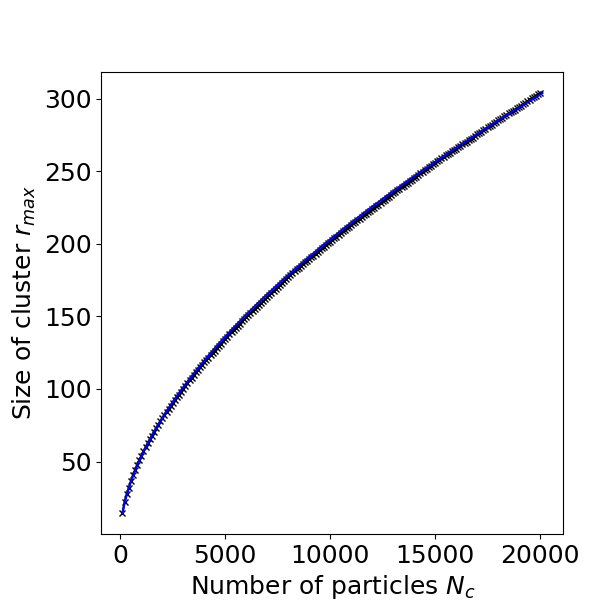
\includegraphics[width=0.95\columnwidth]{100x20k_R.png}
  \caption{
    Mean cluster size $\overbar{r_{max}}$ against particle number $N_c$ over a sample of 100 randomly generated DLA clusters. Error bars representing the 95\% confidence interval on the mean of $r_{max}$ are comparable to symbol sizes and omitted for clarity. The mean fractal dimension $\overbar{d_f}$ of the 100 cluster sample is found to be 1.733$\pm$0.004. Overlaid in blue is a plot of $N_c={\overbar{r_{max}}}^{\overbar{d_f}}$.
  }
  \label{20k_R}
\end{figure}

  Using the least squares fit method the relationship described in (\ref{dim_relation}) is fit to each DLA cluster generated and the $d_f$ are inferred. We find the mean $\overbar{d_f}$ to be 1.696$\pm$0.044, where the uncertainty includes a correction for fitting error. The mean $d_f$ from the ratio of logarithms method taken at $N_c = 20000$ on each cluster finds $\overbar{d_f} =$ 1.733 $\pm$ 0.004. The validity of the ratio of logarithms result is discussed in the following section. Both measurements agree with other literature which suggest a fractal dimension of $\sim~$1.7 in simulations \cite{Witten_1981, Choi_2011, Ranguelov_2011} and in real physical systems such as dielectric breakdown \cite{Pietronero_1984, Irurzun_2002}. A plot of the mean $r_{max} = \overbar{r_{max}}$ against $N_c$ is shown in FIG \ref{20k_R}, overlaid is a plot of $N_c={\overbar{r_{max}}}^{\overbar{d_f}}$ with the $\overbar{d_f}$ determined by the ratio of logarithms method.

  The least squares fit method has significant drawbacks that are important to consider when interpreting these results. We make the assumtion that the relationship described in (\ref{dim_relation}) holds for all scales: the dummy variables $\alpha$ and $\beta$ are included to allow for corrections, however the least squares procedure will give weight to the data at small $N_c$, which is not as representative of the fractal properties that only appear at larger cluster sizes as $r_{max} >> a=1$. There are ways of mitigating this however, e.g. for a sufficiently large cluster the fit can be applied to data that omits $N_c$ smaller than some cutoff value. Larger clusters require significantly more computation which is why we limit our dataset to just 100 generated clusters of $N_c = 20000$. This computational cost becomes a greater issue in the following section.

  A key property of fractals is their scale invariance, which our DLA model cannot reproduce for clusters of very small particle number $N_c$. This can however be useful in modelling physical systems which do have characteristic length scales and discrete particles such as electrodeposition\cite{Shaikh_2022}. Other models may also generate DLA clusters from circular particles or on non-square grids, for smaller sized clusters this can better emulate Brownian motion due to the increased degrees of freedom. However, in the limit as the cluster size increases these should all be equivalent to the Weiner process / Brownian motion.

\subsection*{Effect of random adhesion on fractal dimension}
To examine the effects of random adhesion on the fractal dimension of DLA clusters a dataset of 100 clusters per sticking probability $P_{stick}\in[0.1, 1]$ with interval 0.1 (1000 clusters total) of size $N_c = 5000$ is generated. The mean dimension is determined as in the previous section, that is $d_f$ are found for each cluster and the mean $\overbar{d_f}$ is taken over the 100 samples at each $P_{stick}$. The result is 10 values of $\overbar{d_f}$ corresponding to each $P_{stick}$. Smaller clusters than in the previous dataset are generated due to the computational cost of generating larger clusters. A smaller dataset of larger clusters was created however the statistical uncertainties in the resulting $\overbar{d_f}$ were too large ($\sim 20\%$) when using the least squares fit method.

\begin{figure}[t]
\centering
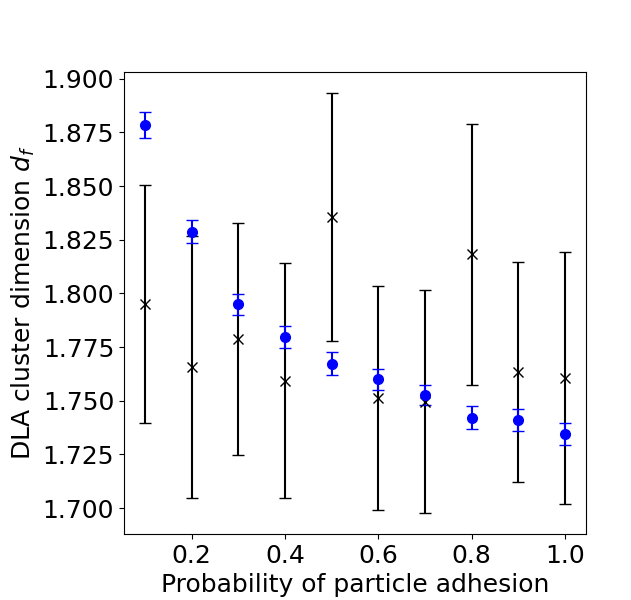
\includegraphics[width=0.95\columnwidth]{stick_dims_together.png}
  \caption{
    Derived mean fractal dimension $\overbar{d_f}$ against sticking probability $P_{stick}$. Two derivations of $\overbar{d_f}$ are shown: in blue $\overbar{d_f}$ is determined by the ratio of logarithms as in (\ref{dim_approx}) by taking the mean $d_f$ at $N_c=5000$ and corresponding $r_{max}$ of each cluster; in black $\overbar{d_f}$ is determined by fitting the relationship in (\ref{dim_relation}) to each cluster and taking the mean. In both error bars represent a 95\% confidence interval on the mean.
  }
  \label{stick_dims_together}
\end{figure}

  Both the least squares fit method and ratio of logarithms method of deriving $d_f$ are applied to this data, a comparison between the two can be seen in FIG \ref{stick_dims_together}. We can observe some striking differences in the derived $\overbar{d_f}$ between the two methods: for $P_{stick}=1$ both methods are able to reproduce within error the ratio of logarithms $\overbar{d_f}$ determined in the previous section. On this dataset at $P_{stick} = 1$ the ratio of logarithms finds $\overbar{d_f} =$ 1.735 $\pm$ 0.005 and the least squares fit finds $\overbar{d_f} = $ 1.761 $\pm$ 0.059. Note that the least squares fit method cannot reproduce its own results within error, this harms its validity.
  
  From the least squares fit method (shown in black in FIG \ref{stick_dims_together}) we see measurements of $\overbar{d_f}$ with no clear correlation, outlier values that deviate from the expected trend, and significant uncertainty. No reasonable conclusion about correlation between $d_f$ and $P_{stick}$ can be drawn from these results. On the other hand, the ratio of logarithms method shows a clear negative correlation between $d_f$ and $P_{stick}$ in line with the results of Ranguelov \textit{et al} \cite{Ranguelov_2011}. The validity of this method should not be taken for granted however, as it relies on the assumtion that measurements taken are in the limit $r_{max} >> a=1$. The small clusters in this dataset have $r_{max} \sim 10^2 \times a$, which seems to be sufficient for this approximation.

  An intuitive interpretation of this negative correlation is that: when a particle fails to adhere in a denser region of the cluster, its subsequent random motion is more likely to collide with another nearby cluster particle. This means denser 'branches' will grow faster than less dense regions in the cluster. This also allows particles to diffuse towards the centre of the cluster and fill in gaps, where they otherwise would have been 'captured' nearer to the starting radius $r_{start}$ \cite{Ranguelov_2011}. These effects overall increase the density of the generated cluster, and thus its fractal dimension.

\section*{Conclusion}

  By comparing the two methods of deriving $d_f$ over varying $P_{stick}$ and critically evaluating the results they produce, we conclude that the ratio of logarithms method is superior to the least squares fit method. The least squares fit method is unsuitable for determining $d_f$ under the conditions we have applied it because of its large statistical uncertainty and inability to reproduce its own results between similar datasets. As such, we will disregard the results from the least squares fit method in our following conclusions. In particular we will disregard its determined fractal dimension for $P_{stick} = 1$ and the lack of correlation between $\overbar{d_f}$ and $P_{stick}$ shown in FIG \ref{stick_dims_together}.

  Using the ratio of logarithms method we determin the fractal dimension of DLA clusters with sticking probability $P_{stick} = 1$ to be $\overbar{d_f} =$ 1.733 $\pm$ 0.004. Additionally we find a negative correlation between the fractal dimension $d_f$ and sticking probability $P_{stick}$ in concurrence with the literature \cite{Ranguelov_2011, Pietronero_1984}. This shows that simple changes to the DLA algorithm can have significant effects on the properties of the resulting clusters.
  
  An example application of the modified probability of adhesion algorithm to a physical system is Pietronero and Wiesmann's model for dielectric breakdown \cite{Pietronero_1984}. In the model, they give the probability of adhesion as a function of the local electric field by some relation coefficient. Their findings also show a negative correlation between fractal dimension and adhesion probability.

  Ranguelov \textit{et al} also make modifications to the radius at which the particles are generated $r_{start}(\theta)$ by setting it as a function of the radius of the cluster at angle $\theta$ + a constant. They also introduce multiple species of particles which have different probabilities of attaching to each other. The resulting clusters can vary drastically in shape and dimension. Their findings provide examples of further modifications that can be made to a DLA system to produce new fractals or better adapt the DLA algorithm to model natural phenomena.

  Further improvements could be made to our results by sampling many more clusters, and clusters of larger sizes to reduce our statistical error. This would also justify further improvements to our implementation of the algorithm that increase computational efficiency. With improving understanding of fractals and DLA systems we can hope to better model the natural processes in which they are seen.

\section*{Acknowledgements}
We would like to acknowledge the contributions of Dr A. Souslov and Dr D. Tsang for their code and resources on which the unmodified DLA model is based.

%%%References
\bibliographystyle{ieeetr}
%bibliographystyle{bathx}
\bibliography{refs}

\clearpage

\onecolumn

\section*{Appendix}

\subsection*{Example DLA clusters}

\begin{figure}[h!]
\centering
  \begin{subfigure}[t]{0.45\textwidth}
    \centering
    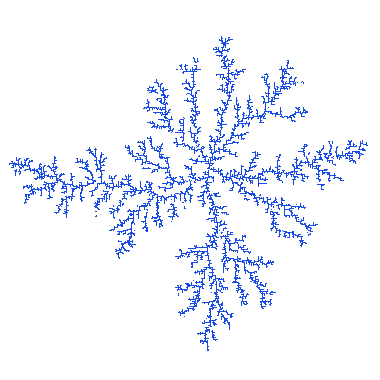
\includegraphics[width=0.95\textwidth]{p1.png}
    \caption{$P_{stick} = 1$}
  \end{subfigure}
  \hfill
  \begin{subfigure}[t]{0.45\textwidth}
    \centering
    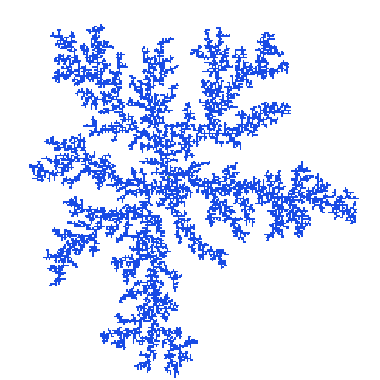
\includegraphics[width=0.95\textwidth]{p01.png}
    \caption{$P_{stick} = 0.1$}
  \end{subfigure}
  \caption{
    Example DLA clusters generated to $N_c = 10000$.
  }
\end{figure}

\subsection*{Confidence intervals}
  For the mean quantities in this report error is presented as the 95\% confidence interval on the mean given by
  \begin{equation}
    a = 1.96\frac{1}{\sqrt{n}}\sigma_x
  \end{equation}
  For some mean quantity $\overbar{x}$ where $\sigma_x$ is the standard deviation on the mean and $n$ is the number of samples. The confidence interval is then $[\overbar{x}-a, \overbar{x}+1]$. This can be interpreted as the interval such that there is a 95\% chance the interval contains the true population mean of $\overbar{x}$.

\subsection*{Implementation of algorithm}
  The DLA data discussed in this report was generated by an implementation of the described DLA algorithm in C++. Standard C++ libraries are used for sampling of 'true' and psuedo-random numbers used in the random walk and particle generation. Utilities were written to record multiple simulations with varying parameters and to export recorded data from simulations to a csv format. Data analysis and derivation of fractal dimension was performed in Python using the numpy and pandas libraries. All computations were performed on a 64-bit desktop processor running Linux Mint 20.1 'Ulyssa'.

  \textbf{Note: when compiling and running the C++ code provided, the makefile in 'source' has been edited. To compile the code place the .cpp and .h files into a directory called 'source' and add in the missing/unedited files (Particle.h, Window.h, Window.cpp). Run 'make -B -C ./source/' from the directory above 'source'. The compiled binary and the data it produces are in this directory, execute the binary using './run'. The python data analysis file 'DLA.py' should also be run from this same directory}

  The changes made to the C++ code given by Dr A. Souslov and Dr D. Tsang are spread throughout the source code provided (i.e: CSVWrite.h, DLASystem.cpp, DLASystem.h, mainDLA.cpp, rnd.h, Makefile). Most of the changes made are used when pressing 't' in the simulation window to set parameters for data recording and $P_{stick}$ etc. Some new functions have been added to the DLASystem class, and a new class CSVWrite is written for data recording. Some select functions are presented here but you would do best to look at the source code with comments.

\begin{lstlisting}
// check if the last particle should stick (to a neighbour)
int DLASystem::checkStick() {
	Particle *lastP = particleList[numParticles - 1];
	int result = 0;
	// loop over neighbours
	for (int i = 0; i < 4; i++) {
		double checkpos[2];
		setPosNeighbour(checkpos, lastP->pos, i);
		// if the neighbour is occupied...
		if (readGrid(checkpos) == 1)
      if(randomStick){
	      double rr = static_cast<double>(rgen.randomInt(1000));
        if (static_cast<double>(rr/1000.0) < stickChance){result = 1;}
        else {result = 0;}
      }
      else {result = 1;}
	}
	return result;
}
\end{lstlisting}

\begin{lstlisting}
void DLASystem::recordData(int numOfSims, int nInterval_, pair<int, int> nRange_) {
  if(running != 0 && !recording){cout << "please pause simulation before recording data" << endl;}
  else{ 
    if (numOfSims >= 2){
      cout << "Starting DLA multiple recording" << endl;
      simNum = numOfSims;
      numSims = numOfSims;
    }else cout << "Starting DLA recording" << endl;
    
    recording = true;

    nInterval = nInterval_;
    nRange = nRange_;
  }
}
\end{lstlisting}

\begin{lstlisting}
//record data on update
void DLASystem::updateRecording() {
  if(numParticles == nRange.second){
    //cout << "recording data at N = " << numParticles << endl;
    numData->push_back(static_cast<double>(numParticles));
    radiusData->push_back(clusterRadius);

    if (simNum == numSims) {dataSet->push_back(*numData);} //only need one column of this

    //when finished in range write data to dataSet \& reset sim
    if (simNum >= 1){
      dataSet->push_back(*radiusData);
      cout << "Sucessfully recorded sim number " << simNum << " data in range (" << nRange.first << ", " << nRange.second << ") with interval " << nInterval << endl;

      //reset initial conditions
      Reset(); //will reset numData and radiusData
      setRandomSeed();
      setFast();

      if (simStickNum != 0 && simNum \% simStickNum == 1 && simNum != numSims){
        if (stickDiff != 0){
          stickChance -= stickDiff;
          if(stickChance<=0){
            cout << "sticking chance is now 0, finishing recording" << endl;
            writeDataCSV();
            recording = false;
            pauseRunning();
          }
          else cout << "new sticking chance set to " << stickChance << endl;
        }
      }

      setRunning();

      if (simNum == 1) {writeDataCSV();}

      simNum--;
      //cout << "conditions reset for simulation number " << simNum << endl;
    }

    if (simNum <= 0) {recording = false; pauseRunning();}
  }
  else if(numParticles > nRange.first
          && numParticles % nInterval == 0
          && numParticles > numData->size() * nInterval + nRange.first){
    //cout << "recording data at N = " << numParticles << endl;
    numData->push_back(static_cast<double>(numParticles)); //dont really need to do this...
    radiusData->push_back(clusterRadius);
  }
}
\end{lstlisting}

\begin{lstlisting}
//write recorded data to a CSV file
void DLASystem::writeDataCSV(){
  auto csv = new CSVWrite("./data.csv");

  csv->WriteVector(dataSet);
  csv->CSVClose();

  //clearDataSet();

  recording = false; //should be false anyways
}
\end{lstlisting}

\end{document}
